\section{Aplicação móvel}

Para este projeto decidimos optar por três páginas web, para tornar a aplicação menos sobrecarregada visualmente e mais interativa do ponto de vista do utilizador.

A página que nos aparece ao iniciar a aplicação chama-se "Adicionar música" (ver \autoref{music}), na qual vamos introduzir o código \ac{rtttl} da respetiva música na primeira caixa de texto e depois pressionamos o botão em baixo para podermos enviar o código para o servidor.

\begin{figure}[htp]
\centering
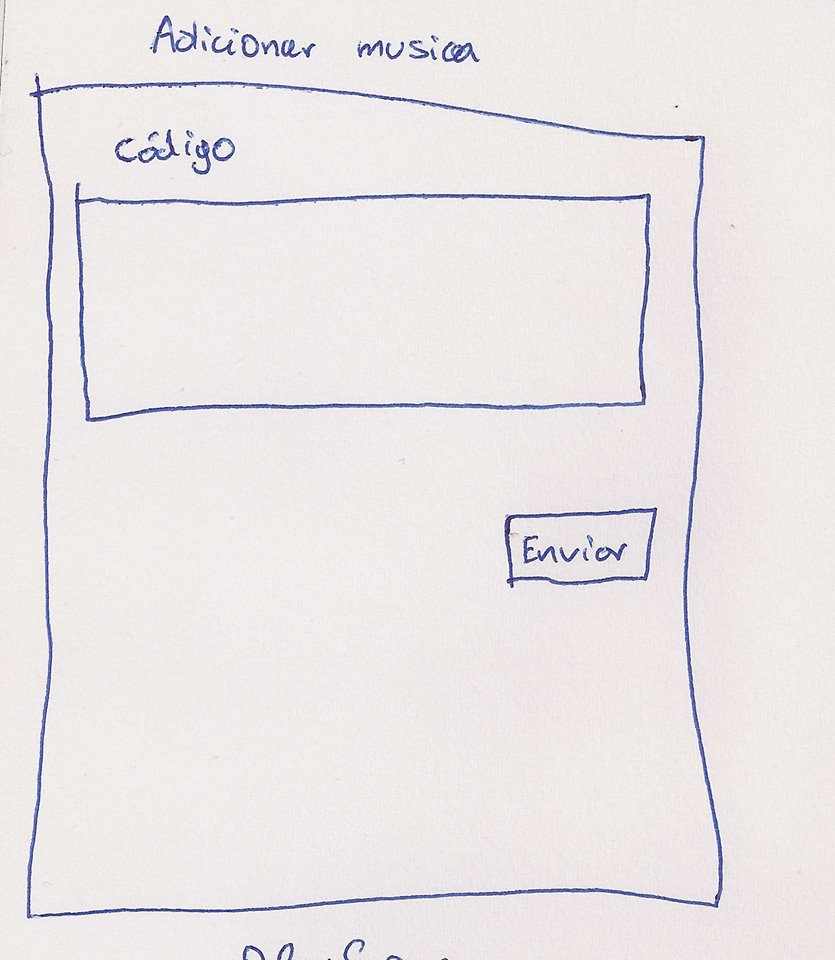
\includegraphics[width=\textwidth]{images/adicionarmusica.jpg}
\caption{Esboço da págna "Adicionar música".}
\label{music}
\end{figure}

Na página "Adicionar intepretação" (ver \autoref{inter}), como o nome indica, vamos adicionar uma nova intepretação a uma música. Temos um \textit{dropdown} que nos vai colocar em lista as músicas guardadas, uma caixa de texto para adicionarmos um registo e outro \textit{dropdown} para acrescentar um efeito à nossa escolha, como ilustra a figura. Após estas escolhas, temos de adicionar o nome que queremos dar à intepretação e enviar para o servidor.

\begin{figure}[htp]
\centering
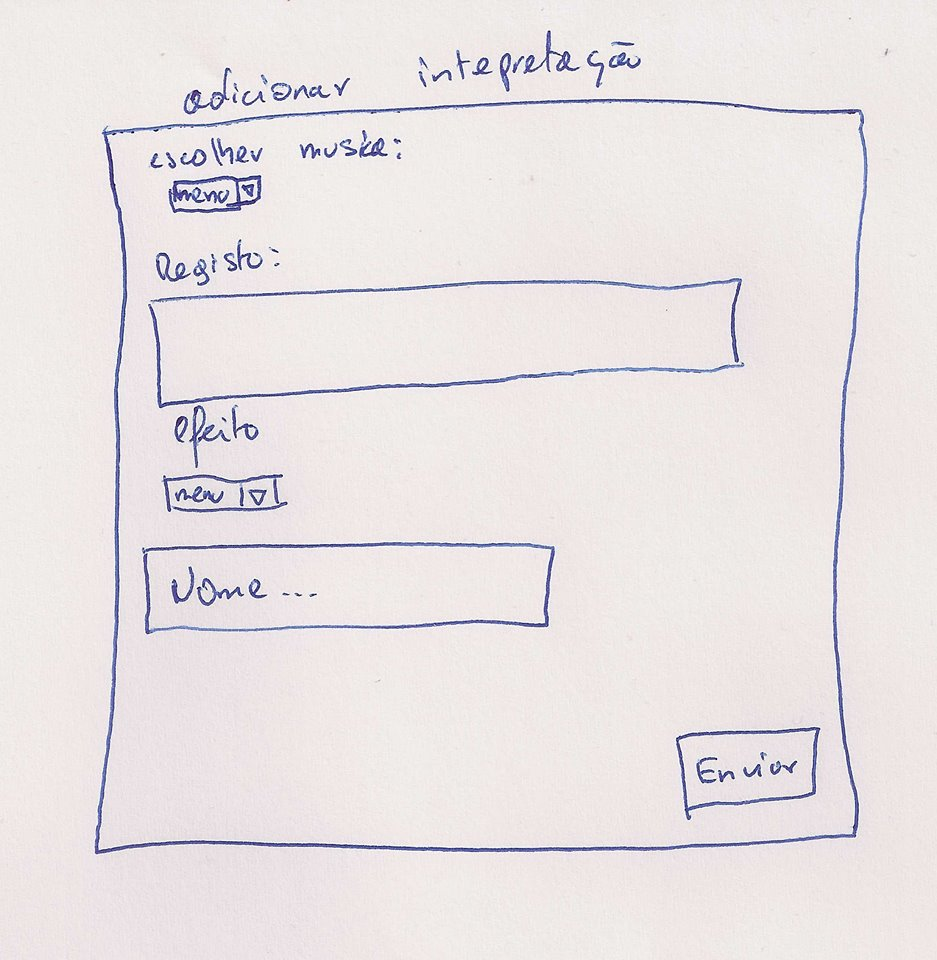
\includegraphics[width=\textwidth]{images/adicionarinterpretacao.jpg}
\caption{Esboço da págna "Adicionar interpretação".}
\label{inter}
\end{figure}

Finalmente, temos a página "Reproduzir música" (ver \autoref{play}), na qual vamos fazer essencialmente reproduzir música. Para isso temos de escolher a música num \textit{dropdown}, escolher a intepretação e carregar no \textit{play}. Ao lado de cada intepretação temos uma barra de gostos/não gostos para classificar cada música.

\begin{figure}[htp]
\centering
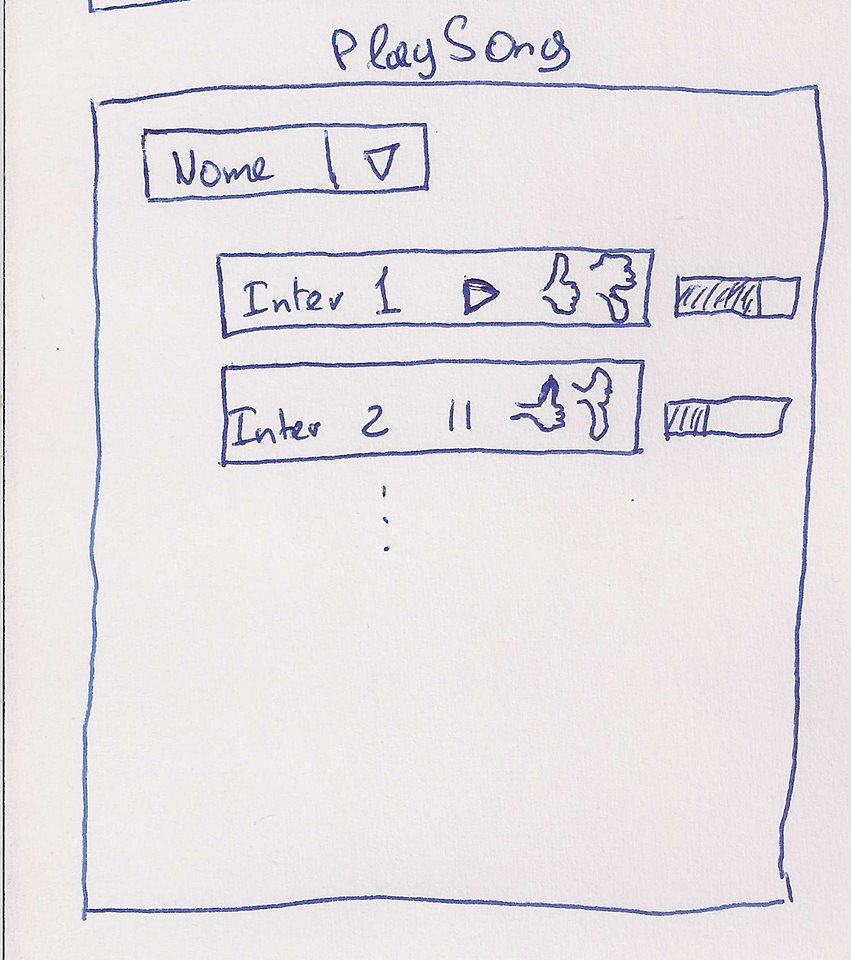
\includegraphics[width=\textwidth]{images/playsong.jpg}
\caption{Esboço da págna "Play song".}
\label{play}
\end{figure}

No decorrer do projeto vamos adicionar mais alguns botões e \textit{navbars} de modo a facilitar a navegação pela \textit{app}.